\usetikzlibrary{calc}

\tikzset{
% Two node styles for game trees: solid and hollow
solid node/.style={circle,draw,inner sep=1.5,fill=black},
hollow node/.style={circle,draw,inner sep=1.5},
square node/.style={rectangle,draw, inner sep = 1, fill = black}
}

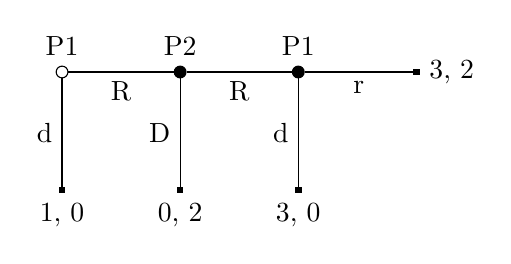
\begin{tikzpicture}[]
  \node[hollow node, label=above:{P1}] {}
    child[grow=right] {
      node[solid node, label=above:{P2}] {}
      child[grow=right] {
        node[solid node, label=above:{P1}] {}
        child[grow=right] {
          node[square node, label=right:{3, 2}] {}
          edge from parent
          node[below] {r}
        }
        child[grow=down] {
          node[square node, label=below:{3, 0}] {}
          edge from parent
          node[left] {d}
        }
        edge from parent
        node[below] {R}
      }
      child[grow=down]  {
        node[square node, label=below:{0, 2}] {}
        edge from parent
        node[left] {D}
      }
      edge from parent
      node[below] {R}
    }
    child[grow=down]  {
      node[square node, label=below:{1, 0}] {}
      edge from parent
      node[left] {d}
    };
\end{tikzpicture}